\documentclass[12pt,letterpaper]{article}
\usepackage{graphicx,textcomp}
\usepackage{natbib}
\usepackage{setspace}
\usepackage{fullpage}
\usepackage{color}
\usepackage[reqno]{amsmath}
\usepackage{amsthm}
\usepackage{fancyvrb}
\usepackage{amssymb,enumerate}
\usepackage[all]{xy}
\usepackage{endnotes}
\usepackage{lscape}
\newtheorem{com}{Comment}
\usepackage{float}
\usepackage{hyperref}
\newtheorem{lem} {Lemma}
\newtheorem{prop}{Proposition}
\newtheorem{thm}{Theorem}
\newtheorem{defn}{Definition}
\newtheorem{cor}{Corollary}
\newtheorem{obs}{Observation}
\usepackage[compact]{titlesec}
\usepackage{dcolumn}
\usepackage{tikz}
\usetikzlibrary{arrows}
\usepackage{multirow}
\usepackage{xcolor}
\newcolumntype{.}{D{.}{.}{-1}}
\newcolumntype{d}[1]{D{.}{.}{#1}}
\definecolor{light-gray}{gray}{0.65}
\usepackage{url}
\usepackage{listings}
\usepackage{color}

\definecolor{codegreen}{rgb}{0,0.6,0}
\definecolor{codegray}{rgb}{0.5,0.5,0.5}
\definecolor{codepurple}{rgb}{0.58,0,0.82}
\definecolor{backcolour}{rgb}{0.95,0.95,0.92}

\lstdefinestyle{mystyle}{
	backgroundcolor=\color{backcolour},   
	commentstyle=\color{codegreen},
	keywordstyle=\color{magenta},
	numberstyle=\tiny\color{codegray},
	stringstyle=\color{codepurple},
	basicstyle=\footnotesize,
	breakatwhitespace=false,         
	breaklines=true,                 
	captionpos=b,                    
	keepspaces=true,                 
	numbers=left,                    
	numbersep=5pt,                  
	showspaces=false,                
	showstringspaces=false,
	showtabs=false,                  
	tabsize=2
}
\lstset{style=mystyle}
\newcommand{\Sref}[1]{Section~\ref{#1}}
\newtheorem{hyp}{Hypothesis}

\title{Problem Set 3}
\author{Erica Lundt}

\begin{document}
	\maketitle
	\section*{Instructions}
	\begin{itemize}
		\item Please show your work! You may lose points by simply writing in the answer. If the problem requires you to execute commands in \texttt{R}, please include the code you used to get your answers. Please also include the \texttt{.R} file that contains your code. If you are not sure if work needs to be shown for a particular problem, please ask.
	\item Your homework should be submitted electronically on GitHub.
	\item This problem set is due before 23:59 on Thursday November 12, 2026. No late assignments will be accepted.

	\end{itemize}

		\vspace{.25cm}
	
\noindent In this problem set, you will run several regressions and create an add variable plot (see the lecture slides) in \texttt{R} using the \texttt{incumbents\_subset.csv} dataset. Include all of your code.

	\vspace{.5cm}
\section*{Question 1}
\vspace{.25cm}
\noindent We are interested in knowing how the difference in campaign spending between incumbent and challenger affects the incumbent's vote share. 
	\begin{enumerate}
		\item Run a regression where the outcome variable is \texttt{voteshare} and the explanatory variable is \texttt{difflog}.
			\lstinputlisting[language=R, firstline=43, lastline=44, breaklines=true]{PS03_EL.R}	
			
			
		 \textit\textbf{{\textbf{EXPLANATION OF REGRESSION}: Holding all things constant, on average for every unit increase in difference in campaign spending, the incumbent and challenger's vote share increases by .042. 	} }
		
		\item Make a scatterplot of the two variables and add the regression line. 
		\lstinputlisting[language=R, firstline=48, lastline=53, breaklines=true]{PS03_EL.R}	
		
	\begin{figure}[H]
		\centering
		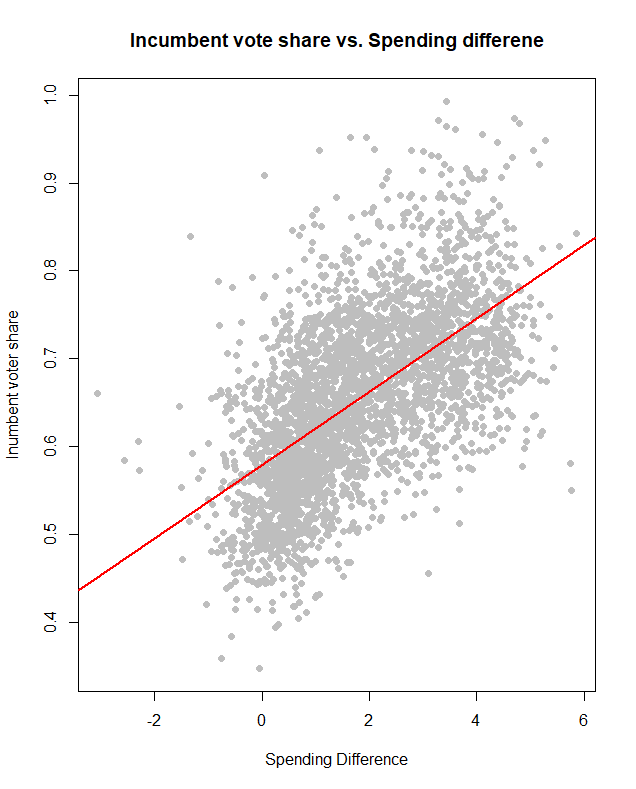
\includegraphics[width=0.8\textwidth]{Plot1_EL.png}
		\caption{Incumbent Vote Share vs Spending.}
		\label{fig:iq-plot}
	\end{figure}
		
		\item Save the residuals of the model in a separate object.
		
		\lstinputlisting[language=R, firstline=55, lastline=63, breaklines=true]{PS03_EL.R}
		
	\begin{table}[!htbp] \centering 
		\caption{Summary of Residuals} 
		\label{} 
		\begin{tabular}{@{\extracolsep{5pt}}lccccc} 
			\\[-1.8ex]\hline 
			\hline \\[-1.8ex] 
			Statistic & \multicolumn{1}{c}{N} & \multicolumn{1}{c}{Mean} & \multicolumn{1}{c}{St. Dev.} & \multicolumn{1}{c}{Min} & \multicolumn{1}{c}{Max} \\ 
			\hline \\[-1.8ex] 
			Residuals & 3,193 & $-$0.0000 & 0.0787 & $-$0.2683 & 0.3275 \\ 
			\hline \\[-1.8ex] 
		\end{tabular} 
	\end{table} 
	
		\item Write the prediction equation.
		
		\ \textit\textbf{{\textbf{ANSWER}: voteshare = 0.58 + 0.042 * difflog 	} }
	\end{enumerate}
	
\newpage

\section*{Question 2}
\noindent We are interested in knowing how the difference between incumbent and challenger's spending and the vote share of the presidential candidate of the incumbent's party are related.	\vspace{.25cm}
	\begin{enumerate}
		\item Run a regression where the outcome variable is \texttt{presvote} and the explanatory variable is \texttt{difflog}.
		\lstinputlisting[language=R, firstline=69, lastline=70, breaklines=true]{PS03_EL.R}	
		
		\textit\textbf{{\textbf{EXPLANATION OF REGRESSION}: Holding all things constant, on average for every unit increase in difference in campaign spending, the presidential candidate vote share for the incumbent's party increases by .023. 
			} }
		
		
		\item Make a scatterplot of the two variables and add the regression line. 	
		
		\lstinputlisting[language=R, firstline=75, lastline=80, breaklines=true]{PS03_EL.R}	
		
		\begin{figure}[H]
			\centering
			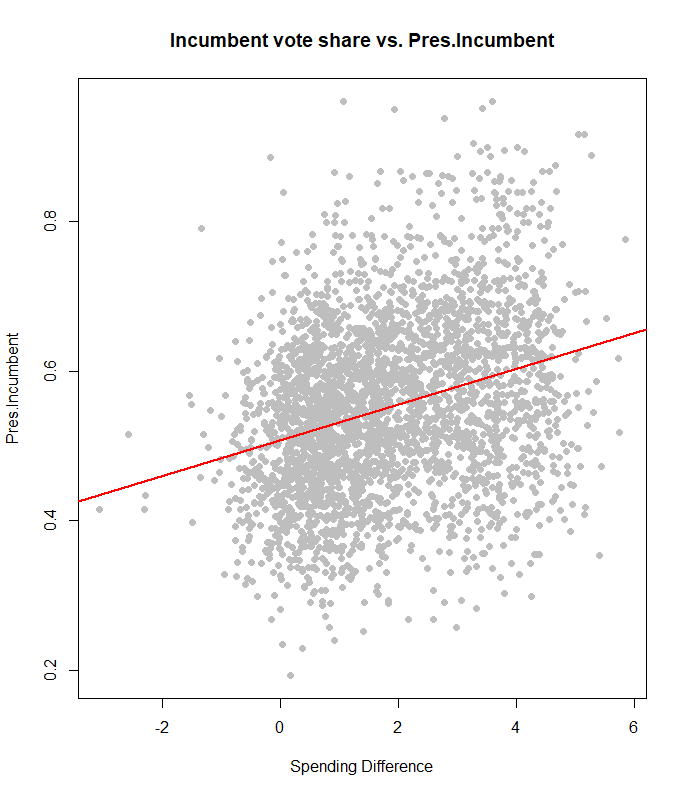
\includegraphics[width=0.8\textwidth]{Plot2_EL.png}
			\caption{President Incumbent Party vs Spending.}
			\label{fig:iq-plot}
		\end{figure}
		
		
		\item Save the residuals of the model in a separate object.	
			\begin{table}[!htbp] \centering 
			\caption{Summary of Residuals} 
			\label{} 
			\begin{tabular}{@{\extracolsep{5pt}}lccccc} 
				\\[-1.8ex]\hline 
				\hline \\[-1.8ex] 
				Statistic & \multicolumn{1}{c}{N} & \multicolumn{1}{c}{Mean} & \multicolumn{1}{c}{St. Dev.} & \multicolumn{1}{c}{Min} & \multicolumn{1}{c}{Max} \\ 
				\hline \\[-1.8ex] 
				Residuals & 3,193 & 0.0000 & 0.1104 & $-$0.3220 & 0.4274 \\ 
				\hline \\[-1.8ex] 
			\end{tabular} 
		\end{table} 
		
		\lstinputlisting[language=R, firstline=83, lastline=89, breaklines=true]{PS03_EL.R}	
		
		
		\item Write the prediction equation.
		
		\ \textit\textbf{{\textbf{ANSWER}: voteshare = -0.21 + .023 * presvote	} }
	\end{enumerate}
	
	\newpage	
\section*{Question 3}

\noindent We are interested in knowing how the vote share of the presidential candidate of the incumbent's party is associated with the incumbent's electoral success.
	\vspace{.25cm}
	\begin{enumerate}
		\item Run a regression where the outcome variable is \texttt{voteshare} and the explanatory variable is \texttt{presvote}.
				\lstinputlisting[language=R, firstline=96, lastline=97, breaklines=true]{PS03_EL.R}	
			
			\textit\textbf{{\textbf{EXPLANATION OF REGRESSION}: Holding all things constant, on average for every unit increase of the vote share, the presidential candidate vote share for the incumbent's party increases by .38
					
			} }
			
			
		\item Make a scatterplot of the two variables and add the regression line. 
		
		\lstinputlisting[language=R, firstline=101, lastline=106, breaklines=true]{PS03_EL.R}
		
	\begin{figure}[H]
		\centering
		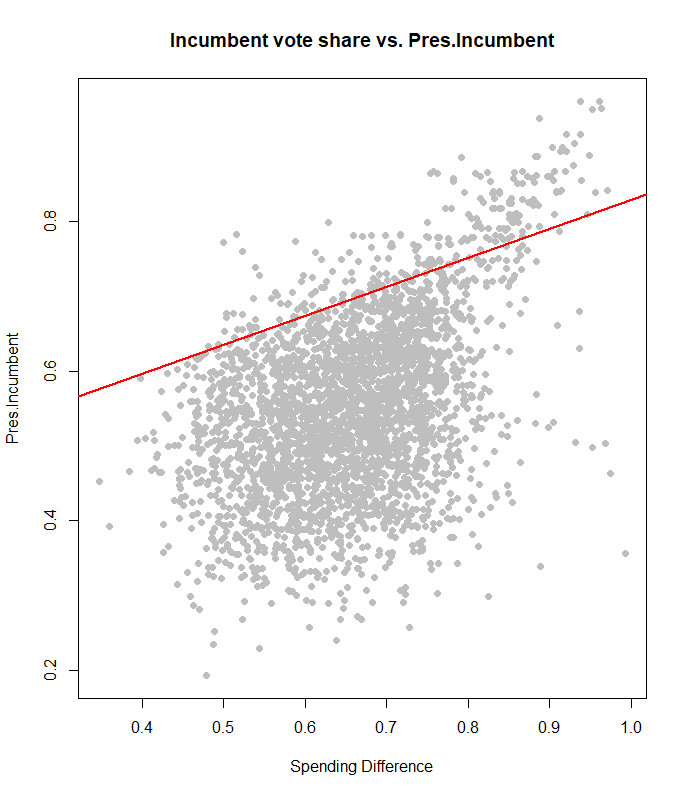
\includegraphics[width=0.8\textwidth]{Plot3_EL.png}
		\caption{Incumbent Vote Share vs President Incumbent Party.}
		\label{fig:iq-plot}
	\end{figure}
		
		\item Write the prediction equation.
		
				\ \textit\textbf{{\textbf{ANSWER}: voteshare = .044 + .38 * voteshare	} }
		
	\end{enumerate}
	

\newpage	
\section*{Question 4}
\noindent The residuals from part (a) tell us how much of the variation in \texttt{voteshare} is $not$ explained by the difference in spending between incumbent and challenger. The residuals in part (b) tell us how much of the variation in \texttt{presvote} is $not$ explained by the difference in spending between incumbent and challenger in the district.
	\begin{enumerate}
		\item Run a regression where the outcome variable is the residuals from Question 1 and the explanatory variable is the residuals from Question 2.
		
			\lstinputlisting[language=R, firstline=117, lastline=118, breaklines=true]{PS03_EL.R}
			
		\item Make a scatterplot of the two residuals and add the regression line.
			\begin{figure}[H]
			\centering
			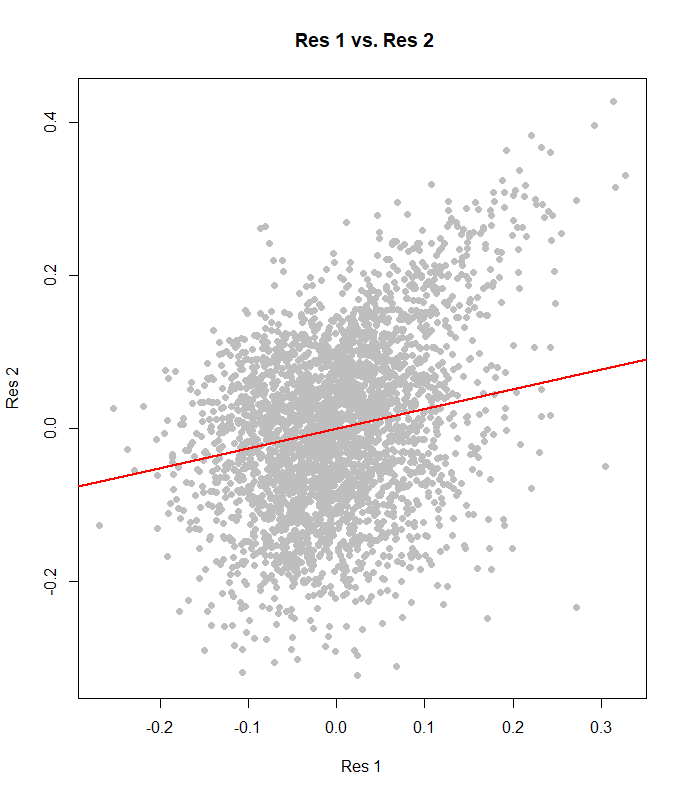
\includegraphics[width=0.8\textwidth]{Plot4_EL.png}
			\caption{Res 1 vs Res2}
			\label{fig:iq-plot}
		\end{figure}
		
		\item Write the prediction equation.
		\textit\textbf{{\textbf{ANSWER}: voteshare = -6.5 + -6.1 * res 1	} }
		
	\end{enumerate}
	
	\newpage	

\section*{Question 5}
\noindent What if the incumbent's vote share is affected by both the president's popularity and the difference in spending between incumbent and challenger? 
	\begin{enumerate}
		\item Run a regression where the outcome variable is the incumbent's \texttt{voteshare} and the explanatory variables are \texttt{difflog} and \texttt{presvote}.
		
			\lstinputlisting[language=R, firstline=133, lastline=134, breaklines=true]{PS03_EL.R}
		
		\item Write the prediction equation.
	\textit\textbf{{\textbf{ANSWER}: voteshare = .44 +.035 X difflog + .25 * presvote	} }
		\item What is it in this output that is identical to the output in Question 4? Why do you think this is the case?
			\textit\textbf{{\textbf{ANSWER}:The residuals for the outputs of questions 4 and 5 are identical. I believe this is because regressing one set of residuals on another isolates the variation that remains unexplained by the other variables. When additional variables are added to the regression, they account for that remaining variation, so the residuals end up the same	} }
		
		
	\end{enumerate}




\end{document}
